%%%%%%%%%%%%%%%%%%%% book.tex %%%%%%%%%%%%%%%%%%%%%%%%%%%%%
%
% sample root file for the chapters of your "monograph"
%
% Use this file as a template for your own input.
%
%%%%%%%%%%%%%%%% Springer-Verlag %%%%%%%%%%%%%%%%%%%%%%%%%%


% RECOMMENDED %%%%%%%%%%%%%%%%%%%%%%%%%%%%%%%%%%%%%%%%%%%%%%%%%%%
\documentclass[graybox,envcountchap,sectrefs]{SVmonoND}

\usepackage{type1cm}
\usepackage{makeidx}         % allows index generation
\usepackage{graphicx}        % standard LaTeX graphics tool
                             % when including figure files
\usepackage{multicol}        % used for the two-column index
\usepackage[bottom]{footmisc}% places footnotes at page bottom
\usepackage{newtxtext}       %
\usepackage[varvw]{newtxmath}% selects Times Roman as basic font
\usepackage{framed}
\usepackage{color}


%%% Norman Dunbar's settings.
%%%==========================================================================%%%
%%%              Packages and such like added by Norman Dunbar               %%%
%%%==========================================================================%%%

\usepackage{nameref}% To use \nameref{...}
\usepackage{wrapfig}% To wrap text around figures.
\usepackage{listings}% Guess!
\usepackage[toc,page]{appendix}% Gets a ``blank'' Appendix page.
\usepackage{longtable}% For tables extending over a page.
\usepackage[obeyspaces]{url}% Allow spaces in \path{}.
\usepackage{xurl}% Ensure \URLs break at /.:*-~'" characters.
\usepackage{xcolor}% Required for the setup of the listings.
\usepackage[LGR,T1]{fontenc}% To get Ohms symbols.
\usepackage{array}%To get table's centred and wrapped.
\usepackage{courier}% For listings, the default is dire!
\usepackage[unicode=true,
    bookmarks=true,
    bookmarksnumbered=false,
    bookmarksopen=false,
    breaklinks=true,
    pdfborder={0 0 0},
    pdfborderstyle={},
    backref=false,
    colorlinks=true]{hyperref}
\usepackage{multicol}
\usepackage{multirow}
\usepackage{pmboxdraw} % For `tree` diagrams.

\urlstyle{same}% Ensure URLs are in the same font as the text. Not in monotype!

\definecolor{ocre}{RGB}{243,102,25}
\definecolor{wwwDarkGreen}{HTML}{006400}
\definecolor{wwwDarkOrchid}{HTML}{9932CC}
\definecolor{wwwDarkOrange}{HTML}{FF8C00}


\input{arduinoLanguage.tex}% To get Arduino code highlighting

\lstdefinestyle{myArduino}{%% Define an Arduino style for use later %%
    language=Arduino,
    %% Add other words needing highlighting below %%
    morekeywords=[1]{},                  % [1] -> dark green
    morekeywords=[2]{FILE_WRITE},        % [2] -> light blue
    morekeywords=[3]{SD, File},          % [3] -> bold orange
    morekeywords=[4]{open, exists},      % [4] -> orange
    %% The lines below add a nifty box around the code %%
    frame=single,
    rulesepcolor=\color{arduinoBlue},
    numbers=left,
    basicstyle={\footnotesize\ttfamily}%To match lstlisting settings
}

\input{AVRAssemblyLanguage.tex}

\lstdefinestyle{AVRasm}{
    language=AVRAssembly,
    %% Add other words needing highlighting below %%
    morekeywords=[1]{},        % [1] -> dark blue - opcodes
    morekeywords=[2]{},        % [2] -> blue - registers & bit names
    morekeywords=[3]{},        % [3] -> bold orange - directives
    morekeywords=[4]{},        % [4] -> bold green - assembler functions
    %% The lines below add a nifty box around the code %%
    frame=single,
    rulesepcolor=\color{arduinoBlue},
    numbers=left,
    basicstyle={\footnotesize\ttfamily}%To match lstlisting settings
}

% Macros for Arduino Assembly Language.
\newcommand{\ardvers}{2.1.0}%VEesion of Arduino IDE in use.

\newcommand{\ohms}{\textgreek{W}}%Ohms symbol.
\newcommand{\app}[1]{\emph{#1}}%Application names.
\newcommand{\reg}[1]{\texttt{\uppercase{#1}}}%Register names.
\newcommand{\regmc}[1]{\texttt{#1}}%Register names.
\newcommand{\regbit}[1]{\texttt{\uppercase{#1}}}%Register bit names.
\newcommand{\bin}[1]{0b{#1}}%Binary numbers.
\newcommand{\hexa}[1]{0x\uppercase{{#1}}}%Hexadecimal numbers.
\newcommand{\varb}[1]{\texttt{#1}}%Variable names.
\newcommand{\code}[1]{\texttt{#1}}%Inline code segments.
\newcommand{\func}[1]{\texttt{#1}}%Procedure and function names.
\newcommand{\pin}[1]{\texttt{#1}}%Arduino/AVR pin names.
\newcommand{\unitname}[1]{\texttt{#1}}%ELF section names.
\newcommand{\externC}{\code{extern \textquotedbl{}C\textquotedbl}}
\newcommand{\shl}{\texttt{<}\texttt{<}~}% << in inline code.
\newcommand{\shr}{\texttt{>}\texttt{>}~}% >> in inline code.
\newcommand{\atmega}{ATmega328P}% Get capitalisation correct!
\newcommand{\lyxarrow}{$\rightarrow$}
\newcommand{\twi}{I$^2$C}


%%% Setup Hyperref configuration %%%
\hypersetup{pdftitle={Arduino Assembly Language},
    pdfauthor={Norman Dunbar},
    pdfsubject={Using AVR Assembly Language with the Arduino IDE.},
    pdfkeywords={Arduino, AVR, ATmega328P,  microcontroller, Uno, Duemilanove, Nano, Assembly Language}}


%%% Lyx specific additions %%%
\makeatletter

\DeclareRobustCommand{\greektext}{%
    \fontencoding{LGR}\selectfont\def\encodingdefault{LGR}}
\DeclareRobustCommand{\textgreek}[1]{\leavevmode{\greektext #1}}
\ProvideTextCommand{\~}{LGR}[1]{\char126#1}

\makeatother

%%% Settings for listings %%%
\lstset{breaklines=true,
    tabsize=4,
    basicstyle={\footnotesize\ttfamily}, %%% Overridden by SVMono class. :(
    basewidth={0.55em}, %%% Needed to fit listings on page %%%
    showspaces=false,
    showstringspaces=false,
    keepspaces=true,
    frame=single}

%%%==========================================================================%%%
%%%                End of Norman Dunbar's additions                          %%%
%%%==========================================================================%%%



% see the list of further useful packages
% in the Reference Guide

\makeindex             % used for the subject index
                       % please use the style svind.ist with
                       % your makeindex program

%%%%%%%%%%%%%%%%%%%%%%%%%%%%%%%%%%%%%%%%%%%%%%%%%%%%%%%%%%%%%%%%%%%%%

%\includeonly{
%
%}

\begin{document}

\author{Norman Dunbar}
\title{Writing Arduino Libraries}
\date{June 16, 2026}
\subtitle{A presentation to The T-Exchange, August 2026.}

\maketitle

\frontmatter%%%%%%%%%%%%%%%%%%%%%%%%%%%%%%%%%%%%%%%%%%%%%%%%%%%%%%

\tableofcontents




\mainmatter%%%%%%%%%%%%%%%%%%%%%%%%%%%%%%%%%%%%%%%%%%%%%%%%%%%%%%%

\chapter{Introduction}

In this short chat, I will explain the background processes and files required to write a small library for use with the Arduino IDE---and it can also be used with PlatformIO\footnote{\url{https://platformio.org}} too.

PlatformIO is another IDE system, but very much improved over the Arduino IDE, event with the latest release of the IDE.

The library I develop will be for a small temperature sensor, the LM75A or the LM75B. These devices allow the current temperature to be read; an alarm to be triggered when the temperature exceeds a preset value; amongst other features.

The data sheet for these sensors can be downloaded from \url{https://www.nxp.com/docs/en/data-sheet/LM75B.pdf}.

The LM75 family of sensors communicate with \twi{} aka TWI aka Wire. Wire is the Arduino library used to talk \twi{} but cannot be called \twi{} for copyright reasons!

The LM75 sensors have quite a number of features, but in the interests of all of us getting home tonight, I am limiting the discussion to simply reading the temperature and reading the device product id. I do have an LM75A library which I wrote in Assembly Language for my book \emph{Arduino Assembly Language} coming to the shops in the next couple of months. That library does cover everything that the LM75 sensors have to offer.

\section{What is a Library?}

In a nutshell, a library is something you create when you find yourself writing the same code, over and over again, in different sketches.

Libraries are not specific to the Arduino system, the C and C++ compilers used by the Arduino IDE have their own support libraries so that you, and I, don't have to keep duplicating code.

In addition, the code in a library has \emph{usually} been well tested so by using the library, instead of writing code over and over, you have less chance of making a typing mistake and introducing bugs into your sketches.

\begin{tips}{Tip}
    Write your library code in plain C. That way people who may wish to include your library in a C++ sketch or library, can do so without errors. The same is not true if you write in C++ and someone wants to use it in a C sketch or library.
\end{tips}


\section{Library Background}

When writing libraries, other than the library source itself, there are three other supporting files required by every Arduino Library:

\begin{itemize}
    \item The Library Properties file.
    \item The keywords file.
    \item The licence\footnote{Yes, I know, American spelling!} file.
\end{itemize}

These files will be discussed shortly. First of all, the tree structure for a library is required.

\section{Library Tree Structure}

When developing your library code, it's best to duplicate the exact structure that will be required when the library is installed in the IDE.

For the library I'm developing here today, \path{LM75A_AB} covers both the LM75A and LM75B devices which are pretty much identical if you get them from NXP Semicondictor. Older LM75As are not quite the same, but the code still works. The file structure we need to create is as follows.

You will note the presence of the boilerplate files---\path{LICENSE}, \path{keywords.txt} and \path{library.properties}

\begin{verbatim}
LM75_AB
├── examples
│   └── Temperature
│       └── Temperature.ino
├── keywords.txt
├── library.properties
├── LICENSE
└── src
    ├── LM75_AB.c
    └── LM75_AB.h

3 directories, 6 files
\end{verbatim}

If your library supplies any example sketches, they must be located in the \path{examples} sub-directory. The source files, all of them, has to live in the \path{src} sub-directory and, not shown here, you can provide documentation in a \path{Docs} folder---but it will not show up anywhere in the IDE, it's entirely for you and/or your library users to find and use as appropriate!

The URL \url{https://arduino.github.io/arduino-cli/1.5/library-specification/} has details of what is required when creating new Arduino libraries. This applies to all IDE versions from 1.5 onward.


\chapter{Boilerplate Files}

Any library that you wish to distribute should have the three boilerplate files as noted above. We will start with the easy one---the licence file---named \path{LICENSE}. You will note that it has the American spelling, c'est la vie\footnote{As they say in Cardiff!}

\section{The Licence File}

The \path{LICENSE} file is a simple text file which details how you wish to license the use of your library. In many cases, the \emph{MIT License} is used, which basically gives everyone the rights to use the library as they see fit, in commercial or non-commercial products.

My own libraries, usually published for use with my books, are always licenced under the MIT licence which allows anyone to do anything. It's easiest. Listing \ref{lst: The MIT Licence for the LM75A library} shows an example.

There are other licencing options, and the easiest manner of determining which might be best for your library (or sketch) is to head over to \url{https://choosealicense.com/} and have a look through the options available.

\begin{lstlisting}[caption={The MIT Licence for the LM75\_AB library.},label={lst: The MIT Licence for the LM75A library}]
MIT License

Copyright (c) 2026 Norman Dunbar.

Permission is hereby granted, free of charge, to any person obtaining
a copy of this software and associated documentation files (the
"Software"), to deal in the Software without restriction, including
without limitation the rights to use, copy, modify, merge, publish,
distribute, sublicense, and/or sell copies of the Software, and to
permit persons to whom the Software is furnished to do so, subject to
the following conditions:

The above copyright notice and this permission notice shall be included
in all copies or substantial portions of the Software.

THE SOFTWARE IS PROVIDED ``AS IS'', WITHOUT WARRANTY OF ANY KIND,
EXPRESS OR IMPLIED, INCLUDING BUT NOT LIMITED TO THE WARRANTIES
OF MERCHANTABILITY, FITNESS FOR A PARTICULAR PURPOSE AND
NONINFRINGEMENT. IN NO EVENT SHALL THE AUTHORS OR COPYRIGHT
HOLDERS BE LIABLE FOR ANY CLAIM, DAMAGES OR OTHER LIABILITY,
WHETHER IN AN ACTION OF CONTRACT, TORT OR OTHERWISE, ARISING FROM,
OUT OF OR IN CONNECTION WITH THE SOFTWARE OR THE USE OR OTHER
DEALINGS IN THE SOFTWARE.
\end{lstlisting}

Obviously, if the library is simply for your own use, you don't \emph{need} a \path{LICENSE} file, but it's useful to be explicit from the start. You never know when something will take off!

The licence file is named \path{LICENSE}, in upper case, and must live in the root directory for the library.

Next up, the properties file.

\section{The Library Properties File}

Arduino libraries need a properties file to inform the IDE, and the users, who wrote the library, which microcontrollers and/or frameworks\footnote{A framework is just the collection of libraries, compilers, linkers, assemblers, uploaders and such like that are needed to generate and use sketches for that particular microcontroller you are writing for.} it should be used with and where to get support when it all goes belly up!

In addition, the IDE's \emph{Library Manager} uses it to search and install the library and any dependencies that the library might require.

The URL \url{https://arduino.github.io/arduino-cli/1.5/library-specification/} describes all the permitted fields and how they should be used. You don't need all of them, thankfully!

The properties file I'm using for the LM75\_AB library is shown in Listing \ref{lst: The library properties file for the LM75_AB library}.

\begin{lstlisting}[caption={The \texttt{library.properties} file for the LM75\_AB library.},label={lst: The library properties file for the LM75_AB library}]
name=LM75_AB
version=1.0.0
author=Norman Dunbar <norman@dunbar-it.co.uk>
maintainer=Norman Dunbar <norman@dunbar-it.co.uk>
sentence=LM75A/B temperature sensor routines for Arduino C/C++ code.
paragraph=This library provides various functions for use with LM75A/B temperature sensors in Arduino sketches on ATmega328P and similar AVR/Microchip microcontrollers.
category=Sensors
url=https://github.com/NormanDunbar/LM75_AB
depends=Wire
includes=LM75_AB.h
architectures=avr
dot_a_linkage=true
\end{lstlisting}

The various fields in use for the LM75\_AB library are as follows:

\begin{description}[\textbf{dot\_a\_linkage}]
    \item[\textbf{name}] A simple one! The name of the library as it will be seen in the IDE.
    \item[\textbf{version}] Another easy one, a version number in the format \emph{major.minor.patch}. This is the \emph{semver} or Semantic Versioning format---see \url{https://semver.org} for full details.
    \item[\textbf{author}] The name or nickname of the author(s) and their email addresses (not mandatory) separated by commas if there is more than one author. There's not a comma between the name and the email though, just spaces.
    \item[\textbf{maintainer}] The name and email address of whoever is currently maintaining the library.
    \item[\textbf{sentence}] One sentence explaining what the library is for.
    \item[\textbf{paragraph}] A longer description of the library. Whatever you have for \textbf{sentence} will be prepended to the \textbf{paragraph}, so don't duplicate yourself.
    \item[\textbf{category}] The category, pick one, that the library covers. For LM75\_AB it's a sensor, but you can pick from:
    \begin{itemize}
        \item Display.
        \item Communication.
        \item Signal input/output.
        \item Sensors.
        \item Device control.
        \item Timing.
        \item Data Storage.
        \item Data Processing.
        \item Other.
        \item Uncategorized---which is the default if nothing specified for \textbf{category}.
    \end{itemize}
    \item[\textbf{url}] The URL of the library project. This could be a GitHub repository or a simple website. It will be used when the user clicks ``More Info'' in the Library Manager.
    \item[\textbf{depends}] An optional comma separated list of other libraries that are required to build this library. The Library Manager will use this list to install all the dependencies not already  installed. There's no need to double-quote library names with spaces as the comma is taken as the library name terminating character.
    \item[\textbf{includes}] An optional list of include files that any sketch will require if it is to use your library. Like \textbf{depends} it is a comma separated list. If this is not specified, then all the \path{*.h} files found in the \emph{root source folder}\footnote{What does this actually mean? In the root directory of the library? In the root of the \path{src} directory?} will be included. Be specific and avoid doubt!
    \item[\textbf{architectures}] The architectures that this library, as supplied, can be used on. Unfortunately, there isn't a list on the above URL, so just take a look at any of the supplied libraries for your particular microcontroller to see what they specify.
    \item[\textbf{dot\_a\_linkage}] An optional option. If set to \emph{true}, the library source files will be compiled to an ``archive'' library---\path{Library_name.a}---and then linked to the compiled sketch; if set to \emph{false} then all the source files are compiled to separate \path{*.o} object files and then all are linked with the sketch's \path{sketch.o} to create the \path{sketch.ino.hex}\footnote{Well, not quite! A \path{sketch.ino.elf} is created by the compilation process. Then the \emph{objcopy} utility is executed to convert the \path{sketch.ino.elf} to \path{sketch.ino.hex}---but you get my drift I hope!} file for uploading.
\end{description}

The properties file is named \path{library.properties}, in lower case, and must live in the root directory for the library.

\subsection{The Keywords File}

The \path{keywords.txt} file tells the IDE \emph{at versions prior to 2.0} how to syntax highlight the various keywords used by the library defines, functions, procedures and so on.

It is no longer used with version 2.0 of the IDE and more recent versions. Syntax highlighting in the new IDE is a bit less dependent on the library authors!

You can omit this file for your own libraries, but if you are distributing them for use by others, it's nice to help out those unfortunates who have yet to upgrade to the new IDE!

The \path{keywords.txt} file I'm using for the LM75\_AB library is shown in Listing \ref{lst: The keywords.txt file for the LM75_AB library}.

\begin{lstlisting}[caption={The \texttt{keywords.txt} file for the LM75\_AB library.},label={lst: The keywords.txt file for the LM75_AB library}]
# Syntax Coloring Map

# Classes (KEYWORD1)
# Bold orange highlighting.


# Class Methods & Functions (KEYWORD2)
# Orange highlighting.

LM75_begin	KEYWORD2
LM75_end	KEYWORD2
LM75_setRegister	KEYWORD2
LM75_getProductId	KEYWORD2
LM75_getCurrentTemperature	KEYWORD2


# Others Constants (LITERAL1)
# Light blue highlighting.

# LM75 Registers.
LM75_TEMPERATURE_REG	LITERAL1
LM75_CONFIG_REG	LITERAL1
LM75_T_HYST_REG	LITERAL1
LM75_T_OS_REG 	LITERAL1
LM75_PRODUCT_ID_REG	LITERAL1

# LM75 Configuration bits.
LM75_FAULTS_1	LITERAL1
LM75_FAULTS_2	LITERAL1
LM75_FAULTS_4	LITERAL1
LM75_FAULTS_6	LITERAL1
LM75_OS_POLARITY_LOW	LITERAL1
LM75_OS_POLARITY_HIGH	LITERAL1
LM75_COMPARATOR_MODE	LITERAL1
LM75_INTERRUPT_MODE	LITERAL1
LM75_SHUTDOWN_ENABLE	LITERAL1
LM75_SHUTDOWN_DISABLE	LITERAL1
\end{lstlisting}

\begin{tips}{Warning}
    You must use hard tabs, character \hexa{09}, between the columns. If you use spaces---or if your editor is configured to change hard tabs into a number of spaces---highlighting in the IDE will not work!
\end{tips}

\begin{tips}{Note}
    Although I've shown all the LM75 registers and the various configuration bits, many of those are not used in this simple demo. I have, however, left them in as an ``exercise for the reader''\footnote{These are always author cop-outs!} who may wish to take the library further!
\end{tips}

The \path{keywords.txt} must live in the root directory for the library.
\chapter{LM75 Sensors}

The LM75 is a temperature sensor available from Texas Instruments, amongst others. It is reasonably accurate with a $\pm{2}$\textdegree~C range. It communicates over \twi{} which the Arduino calls ``Wire'' to avoid copyright infringements.

In order for our library to use the Wire library, it must be mentioned in the \textbf{depends} section of the properties file.

The datasheet for the device can be downloaded as a PDF file from \url{https://www.nxp.com/docs/en/data-sheet/LM75B.pdf} or \url{https://www.nxp.com/docs/en/data-sheet/LM75A.pdf} if you have an LM75A variant.

I have included both PDF files in the code repository for this demonstration. You can download everything later.

\section{LM75 Description}

From the LM75B data sheet:

\emph{The LM75B is a temperature-to-digital converter using an on-chip band gap temperature sensor and Sigma-Delta A-to-D conversion technique with an over-temperature detection output. The LM75B contains a number of data registers: Configuration register (\pin{CONF}) to store the device settings such as device operation mode, \pin{OS}\footnote{\pin{OS} is the pin that toggles on over-temperature alarm being activated.} operation mode, \pin{OS} polarity and \pin{OS} fault queue as described in Section 7 of the LM75B data sheet.}

\emph{It also has a temperature register (\pin{Temp}) to store the digital temp reading, and set-point registers (\reg{Tos} and \reg{Thyst}) to store programmable over-temperature shutdown and hysteresis limits, which can be
communicated by a controller via the 2-wire serial I2C-bus interface.}

\emph{The device also includes an open-drain output (\pin{OS}) which becomes active when the temperature exceeds the programmed limits. There are three selectable logic address pins so that eight devices can be connected on the same bus without address conflict.}

\emph{The LM75B can be configured for different operation conditions. It can be set in normal mode to periodically monitor the ambient temperature, or in shutdown mode to minimize power consumption. The \pin{OS} output operates in either of two selectable modes: \pin{OS} comparator mode or \pin{OS} interrupt mode.}

\emph{Its active state can be selected as either HIGH or LOW. The fault queue that defines the number of consecutive faults in order to activate the \pin{OS} output is programmable as well as the set-point limits.
}
\begin{itemize}
    \item \emph{The LM75A and LM75B's temperature register, at least those from NXP Semiconductor, always stores an 11-bit two’s complement value giving a temperature resolution of 0.125\textdegree{}~C.}
    \item \emph{Other LM75A devices, especially older ones, temperature register stores the data as a 9-bit two’s complement value giving a temperature resolution of 0.5\textdegree{}~C.}
\end{itemize}

\emph{This high temperature resolution is particularly useful in applications of measuring precisely the thermal drift or runaway. When the LM75B is accessed the conversion in process is not interrupted (that is, the \twi-bus section is totally independent of the Sigma-Delta converter section) and accessing the LM75B continuously without waiting at least one conversion time between communications will not prevent the device from updating the \reg{Temp} register with a new conversion result. The new conversion result will be available immediately after the Temp register is updated.}

\emph{The LM75B powers up in the normal operation mode with the \pin{OS} pin in comparator mode, temperature threshold of 80\textdegree{}~C and hysteresis of 75\textdegree{}~C\footnote{The temperature that it must cool down to to turn off the alarm.}, so that it can be used as a stand-alone thermostat with those pre-defined temperature set points.}

\emph{Yada, yada, yada!} This is why we need data sheets, it saves typing!

\begin{tips}{Note}
    In \emph{comparator} mode, the \pin{OS} pin will go active when the temperature set in the \reg{TOS} register---default 80\textdegree{}~C---and deactivate when it drops below the temperature set in register \reg{THYST}. Unless catered for, there will be no indication that over-temperature was detected.

    Interrupt mode is slightly more complicated. When an over-temperature is detected, the \pin{OS} pin will activate as above. However, it will stay active for as long as the fault is not cleared by the user or code. This can be used to light an alarm indicator.

    If the fault condition is cleared, then \pin{OS} will deactivate. However, when the temperature drops again below \reg{THYST} it will once again activate.

    These combinations ensure that any fault indicators attached to the \pin{OS} pin will remain lit until cleared manually, even though the fault condition of the over-temperature is no longer active due to temperatures dropping.
\end{tips}

\section{LM75 Features}

These devices are quite capable, provided that $\pm$2--3\textdegree{}~C accuracy is suitable. Briefly:

\begin{itemize}
    \item Works with power supplies between 2.8~V and 5.5~V.
    \item Power use is 1~uA in shutdown (power save) mode. (I have found that this doesn't appear to work and the sensor drawn 10--11~mA in either mode!)
    \item Clock speeds from 20~Hz to 400~KHz can be used.
    \item \twi{} bus with up to eight devices on the bus at any one time.
    \item Temperature range from $-55$\textdegree{}~C to $+125$\textdegree{}~C.
    \item Accurate to $\pm2$\textdegree{}~C from $-25$\textdegree{}~C to $+100$\textdegree{}~C.
    \item Accurate to $\pm3$\textdegree{}~C from $-55$\textdegree{}~C to $+125$\textdegree{}~C.
    \item Over-temperature alarm with user configurable temperature and hysteresis, plus two alarm handling methods.
    \item OS pin can be configured high or low
    \item Product ID and hardware version can be read from the device.
\end{itemize}
\chapter{The \texttt{BareBones.ino} Sketch}

I shall now present you with a small sketch which talks directly with \twi{} to setup, configure and read data from an LM75 sensor. The sketch doesn't make use of many of the features of the sensor, merely these two:

\begin{itemize}
    \item Reading the product id from the LM75. Some LM75s do not have the product id present. I believe only Texas Instruments' devices have it. Mine are NXP Semiconductor.
    \item Reading the current temperature.
\end{itemize}

\section{The Breadboard Layout}

Figure \ref{fig: BareBones.ino - Breadboard layout} (see Page \pageref{fig: BareBones.ino - Breadboard layout}) shows the circuit layout for the \path{BareBones.ino} sketch\footnote{And also, for the \path{WithLibrary.ino} sketch coming later!}.

\begin{figure}[!h]
\begin{centering}
    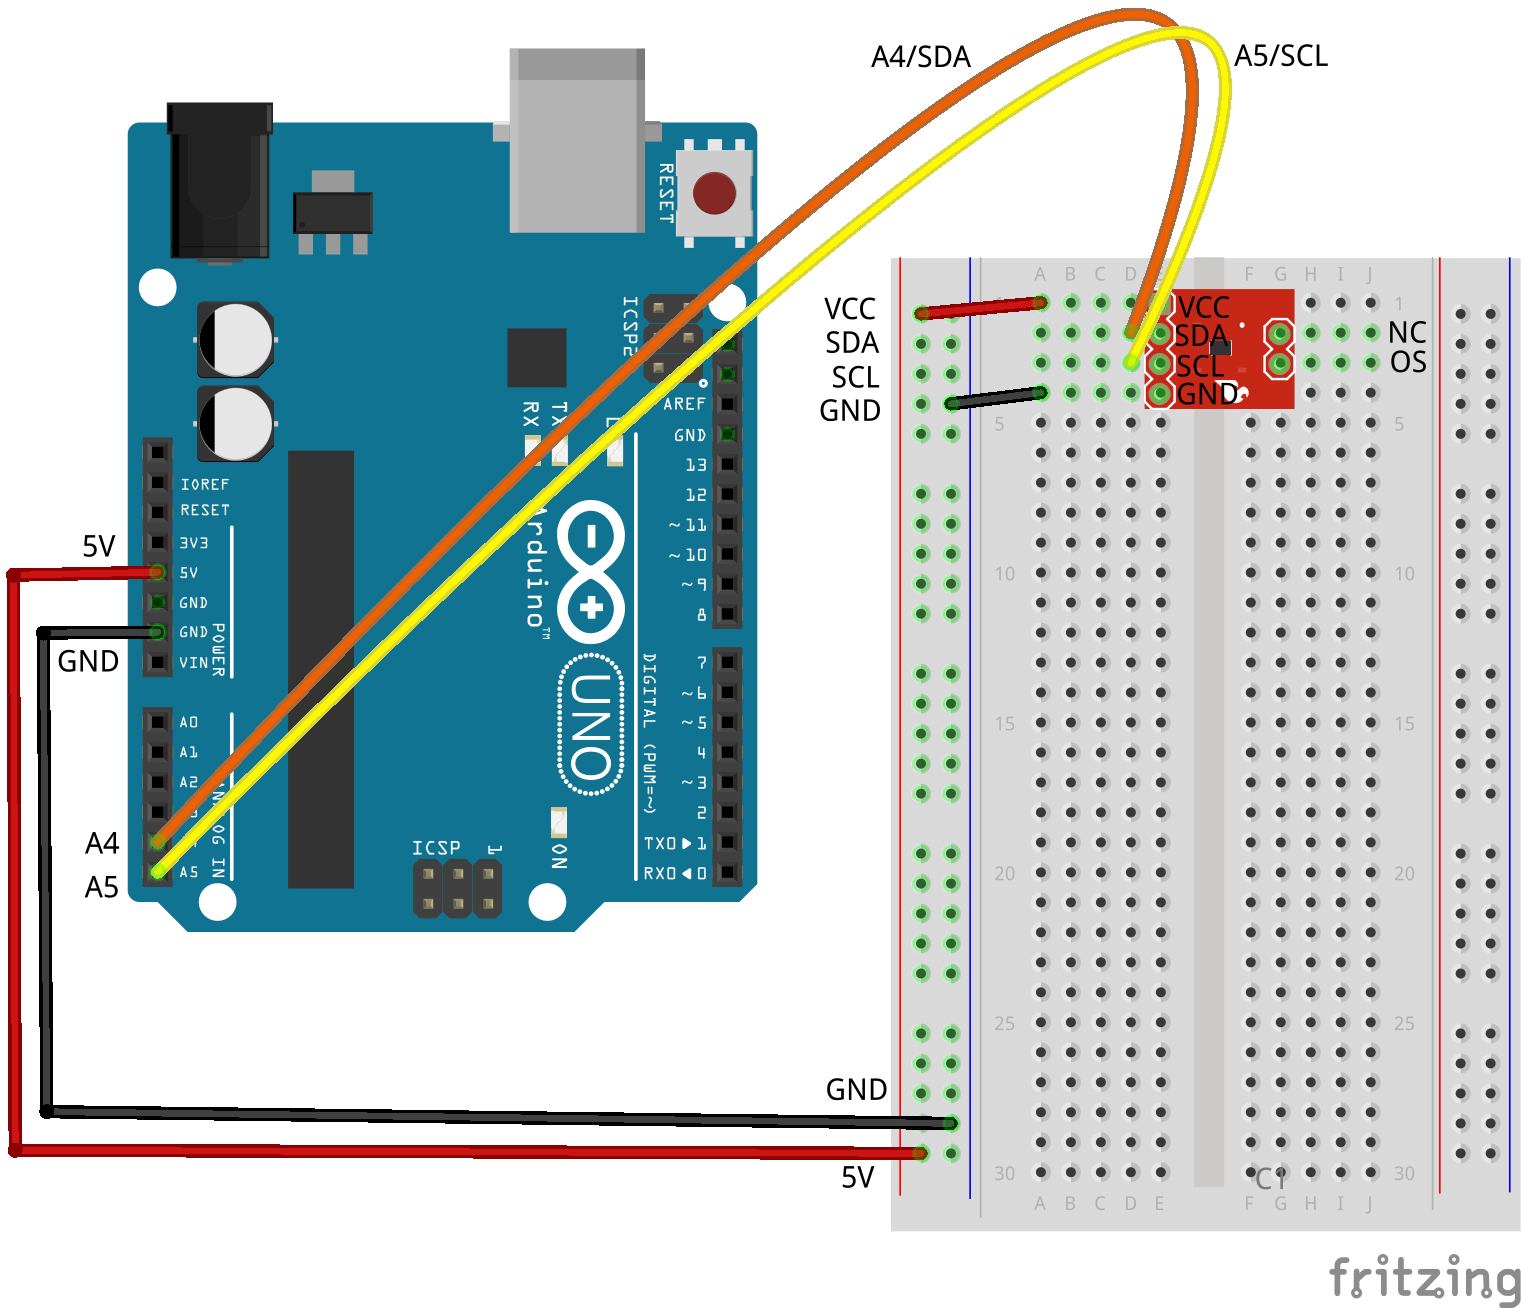
\includegraphics[width=11cm]{Fritzing/BareBones}
    \caption{BareBones.ino - Breadboard layout.}
    \label{fig: BareBones.ino - Breadboard layout}
    \par\end{centering}
\end{figure}

Power and ground connections go directly from the Arduino's power and ground pins, to the supply rails on the breadboard. The sensor's own \pin{VCC} and \pin{GND} pins take their power from the breadboard.

As we are using \twi{}, we have no choice in this matter as it's all the LM75 understands, we need two additional wires---one for the \twi{} bus clock and one for the \twi{} bus data.

On Figure \ref{fig: BareBones.ino - Breadboard layout} you will see the yellow and orange wires are connected to the Arduino's \pin{A5} and \pin{A4} pins respectively.

Other clones of the Arduino Uno, like mine, have two separate pins---\pin{SCL} and \pin{SDA}--- for the \twi{} bus clock and data pins. To avoid confusion, I'm using the same physical layout as shown in Figure \ref{fig: BareBones.ino - Breadboard layout}.

Unfortunately the Fritzing component image is slightly different to my own physical one, but the pins are the same names at least! (\pin{NC} is ``not connected''.)

Right, on with the code.

\section{Sketch Header}

It's always nice to start with a header giving details of what the sketch is doing and when you wrote it. You'd be surprised how often it helps! Here's mine, intentionally kept brief, having said that!

\begin{lstlisting}[caption={BareBones.ino - Header.},label={lst: BareBones.ino - Header}, style=myArduino, firstnumber=1]
//===============================================================
// LM75 Temperature sensor demo for MakerSpace presentation.
//
// Shows how much messing about with I2C/TWI there is in order
// to read the temperature and product id from an LM75A/B sensor.
//
// The LM75A/B can do a lot more than shown here, for the sake of
// brevity, I'm not getting in too deep!
//
//
// Norman Dunbar.
// 16 June 2026.
//===============================================================
\end{lstlisting}

\section{Sketch Prologue}

In the prologue for the sketch, I have included the \path{Wire.h} header file. This is required as I need to access the \twi{} bus.

Following on from that, I have declared the various LM75 accessing functions that will be used in the code. I do it this way as \func{setup()} and \func{loop()} will appear near the top of the listing and should be easier to find when making changes.

The functions declared will be at the bottom of the sketch and as such, the compiler needs to know about them so that when it finds calls to them, it knows how to handle things like parameters and return values.


\begin{lstlisting}[caption={BareBones.ino - Prologue.},label={lst: BareBones.ino - Prologue}, style=myArduino, firstnumber=15]
#include <Wire.h>


// Function prototypes.
void LM75_begin(const int address, uint32_t clockHZ);
void LM75_end();
void LM75_setRegister(const int address, const int reg);
uint8_t LM75_getProductId(const int address);
float LM75_getCurrentTemperature(const int address);


// Where is my sensor?
const int LM75_ADDRESS = 0x4F;

// Bus speed in Hz.
const uint32_t LM75_CLOCK_HZ = 100000;    // 100 KHz.

// LM75 registers.
const int LM75_TEMPERATURE_REG = 0;
const int LM75_PRODUCT_ID_REG = 7;

// Product id is unknown.
const uint8_t LM75_UNKNOWN_ID = 255;
\end{lstlisting}

Following on from the function prototypes, I have made life easy for myself by declaring constants for all the ``magic'' numbers that will appear in the code. If I ever have to make changes, I only need to find and change one value!



\section{Setup}

The Arduino standard \func{setup()} function is next. Not much happens here other than starting the \twi{} bus with a clock speed of 100~KHz and initialising the LM75 sensor attached to address \hexa{4F}---note that this is a seven bit address, not eight!

\eject\begin{tips}{Note}
    Internally, \twi{} uses an eight bit address which is determined by the device's seven bit address shifted left by one bit and a 0 (write) or a 1 (read) tagged onto the lowest bit.

    This gives my particular LM75 sensor a read address of \hexa{4F} \shl{1}|1 which is \hexa{9F}; and a write address of \hexa{4F} \shl{1}|1 which is \hexa{9E}. However, I only have to remember the seven bit address \hexa{4F}.
\end{tips}


\begin{lstlisting}[caption={BareBones.ino - Setup.},label={lst: BareBones.ino - Setup}, style=myArduino, firstnumber=43]
void setup() {
    uint8_t productID;

    // Start up I2C as a controller. Talking to the sensor
    // at 100 KHz.
    LM75_begin(LM75_ADDRESS, LM75_CLOCK_HZ);

    // Need the Serial Monitor for output.
    Serial.begin(9600);
    Serial.println("LM75 Temperature Sensor");
    Serial.print("LM75 Product id: ");

    productID = LM75_getProductId(LM75_ADDRESS);
    if (productID == LM75_UNKNOWN_ID)
    Serial.println("Unknown");
    else
    Serial.println(productID);
}
\end{lstlisting}

After initialising the LM75, Serial is initialised to 9600 baud and a message printed to show that we are starting up. The LM75's product id is fetched from the device and printed---if one is present. See Listing \ref{lst: BareBones.ino - LM75_getProductId} for details.


\section{Loop}

Next up, the Arduino standard \func{loop()} function. Here we simply make a call to the \func{} function, see Listing \ref{lst: BareBones.ino - LM75_getCurrentTemperature}, then print it.


\begin{lstlisting}[caption={BareBones.ino - Loop.},label={lst: BareBones.ino - Loop}, style=myArduino, firstnumber=66]
void loop() {

    // Read the temperature.
    float result = LM75_getCurrentTemperature(LM75_ADDRESS);

    // Print it out with much messing with Serial!
    Serial.print("Temperature: ");
    Serial.print(result);
    Serial.println(" degrees C.");

    // Delay is usually a bad thing, but here we are not doing
    // anything else,
    delay(1500);
}
\end{lstlisting}

Normally, calling \func{delay()} in the \func{loop()}\footnote{Or anywhere else for that matter!} is considered a bad thing. In this case, or in the case of the famous \path{Blink.ino} sketch, there's no other work being done, so it's fine.

The \func{delay()} function, supplied by the Arduino Language, runs a tight loop waiting for a countdown to expire. While it is running, the sketch cannot do anything else\footnote{Unless it receives an interrupt, of course}.

\section{LM75\_begin}

Now we get to the nitty gritty of the LM75 handling functions. Listing \ref{lst: BareBones.ino - LM75_begin} is where we initialise the device and set the \twi{} bus clock to the required speed. The Wire library helps with this.


\begin{lstlisting}[caption={BareBones.ino - LM75\_begin.},label={lst: BareBones.ino - LM75_begin}, style=myArduino, firstnumber=82]
// Initialises the LM75 sensor with a bus speed as required.
void LM75_begin(const int address, uint32_t clockHZ) {
    Wire.begin(address);
    Wire.setClock(clockHZ);
}
\end{lstlisting}

\section{LM75\_end}

Listing \ref{lst: BareBones.ino - LM75_end}, the \func{LM75\_end()} function, is not used in this sketch---the main \func{loop()} never stops using the LM75 sensor, so it never has to call here. If, on the other hand, your sketch code simply accessed the sensor once, or infrequently, then it should release the \twi{} bus between calls so that other \twi{} controller devices can get control of the bus.

\begin{lstlisting}[caption={BareBones.ino - LM75\_end.},label={lst: BareBones.ino - LM75_end}, style=myArduino, firstnumber=88]
// Shuts down the Wire bus for the LM75. This is needed in
// sketches where the bus might be needed by another sensor.
// In this simple demo, it is never called.
void LM75_end() {
    Wire.end();
}
\end{lstlisting}

Once again, all the hard work is done by the Wire library.


\section{LM75\_setRegister}

When we need to switch between reading the product id and the temperature from the LM75, we need to make sure we talk to the correct LM75 register. By default, it powers up with the temperature register active.

As we read the product id first, we need a function to tell the LM75 which register is to be read from, from now on. \func{LM75\_setRegister} does exactly that.

\begin{lstlisting}[caption={BareBones.ino - LM75\_setRegister.},label={lst: BareBones.ino - LM75_setRegister}, style=myArduino, firstnumber=96]
// Configures the LM75 with the register we wish to
// read from, until changed. Ends the write transaction
// when done.
void LM75_setRegister(const int address, const int reg) {
    Wire.beginTransmission(address);
    Wire.write(reg);
    Wire.endTransmission(true);
}
\end{lstlisting}

\func{LM75\_setRegister} starts a write transaction on the \twi{} bus using the Wire library supplied \func{beginTransmission()} function for the LM75's seven bit address address. Internally, it will convert the seven bits to eight with a 0 in  bit zero.

On return, we simply have to write one data byte to the LM75---the register we need to set as the default. The data written by \func{Wire.write()} are queued until we execute \func{endTransmission()}.

The \varb{true} parameter means that the \twi{} bus will end the transaction and release control of the \twi{} bus. This is good etiquette if you have more than one \twi{} device connected to the bus as communication is limited to a single controlling device at any one time.

This is not so important with this sketch as we only have one controlling device, the Arduino itself.


\section{LM75\_getProductId}

The code to retrieve the LM75's product id is shown in Listing \ref{lst: BareBones.ino - LM75_getProductId}. It's quite simple in operation as all it does is to set the default LM75 register to the product id register; read one single data byte back from the LM75 and reset the default LM75 register back to the temperature register.


\begin{lstlisting}[caption={BareBones.ino - LM75\_getProductId.},label={lst: BareBones.ino - LM75_getProductId}, style=myArduino, firstnumber=106]
// Returns the product id byte for the LM75 sensor
// attached. If not present will return 0xFF instead.
uint8_t LM75_getProductId(const int address) {
    uint8_t productID;

    // Select the product id register.
    LM75_setRegister(address, LM75_PRODUCT_ID_REG);

    // Theres only one byte.
    Wire.requestFrom(address, 1, true);

    // Fetch it.
    if (Wire.available())
    productID = Wire.read();

    // Reset default register to temperature.
    LM75_setRegister(address, LM75_TEMPERATURE_REG);

    // Return the product id.
    return productID;
}
\end{lstlisting}

The reason we reset the default register here is to save having to do it \emph{every} time we attempt to read the current temperature. By default, the temperature register is the default register, so we only change away from it when reading the product id. Less code to execute means less chances for errors to occur!

Our Arduino's control of the \twi{} bus will end after the single data byte is read from the LM75 duw to the \varb{true} parameter sent in the function call to \func{Wire.requestFrom()}.

\section{LM75\_getCurrentTemperature}

The function \func{LM75\_getCurrentTemperature()} in Listing \ref{lst: BareBones.ino - LM75_getCurrentTemperature} does all the hard work of reading two bytes from the LM75's temperature register and manipulating them to get a temperature reading in degrees Celcius\footnote{Sorry America, get up to date! ;o)}.

\begin{lstlisting}[caption={BareBones.ino - LM75\_getCurrentTemperature.},label={lst: BareBones.ino - LM75_getCurrentTemperature}, style=myArduino, firstnumber=129]
float LM75_getCurrentTemperature(const int address) {
    // Storage for result
    int8_t tempData[2];
    int16_t result = 0;

    // Two bytes required.
    Wire.requestFrom(address, 2, true);

    // Fetch degrees & fractions as an 11 bit value.
    // Multiply by 0.125 to convert to degrees Celcius.
    if (Wire.available()) {
        tempData[0] = Wire.read();
        tempData[1] = Wire.read() & 0b11100000; // Bits 7--5 only.
        result = ((int16_t)(tempData[0])<<3) + (tempData[1] >> 5);
    }

    return result * 0.125;
}
\end{lstlisting}

The LM75 holds temperature data as an 11 bit value, right aligned in a 16 bit register. When we read the data, the first byte is degrees; the second is fractions of a degree. The top three bits of the second byte hold the fractions:

\begin{itemize}
    \item Bit 7 set is 0.5\textdegree{}~C.
    \item Bit 6 set is 0.25\textdegree{}~C.
    \item Bit 5 set is 0.125\textdegree{}~C.
    \item Bits 4--0 are always zero.
\end{itemize}

The temperature is calculated as the full 11 bit value multiplied by 0.125, with the result in Celsius.


\chapter{The LM75\_AB Library}

I intended to call this library LM75, however, there's already a library by that name---which incidentally, has all the LM75 features implemented---and because it was at a higher version than mine, it downloaded and overwrote mine! Hence the name change.

First a warning!

\begin{tips}{Warning}
    If you write a library which includes the \path{Wire.h} header file in any of the library's own header or source files, you will see compiler errors relating to the \func{class} keyword in the header file \path{Printable.h} amongst many other error messages. This will happen when you attempt to compile a sketch which uses your library.

    \path{Wire.h} is a C++ header and as such, requires the C++ compiler. Your library file is named \path{something.c} so the C compiler is used, and that unfortunately, doesn't know anything about C++ classes.

    The solution is simple. Rename your library's source files from \path{something.c} to \path{something.cpp}
\end{tips}

\section{Creating the Library}

It's much easier, the above warning not withstanding, to create a library from a working sketch. By having a working sketch, you know that your code is working so any problems after conversion to a library, is a problem in the conversion and not in the code.

To convert our sketch to a library, I opened \path{BareBones.ino} and saved it as \path{WithLibrary.ino} then extracted all of the LM75 related functions into the library source file \path{LM75_AB.cpp}; and the various constants and function prototypes into \path{LM75_AB.h}.

\subsection{Header File \texttt{LM75\_AB.h}}

As mentioned above, all I've done to create the header file is extract all the constants and functions that relate purely to the LM75 accesses. We don't want any sketch specific constants here, only those of the LM75.

\begin{lstlisting}[caption={Library header file - \texttt{LM75\_AB.h}.},label={lst: LM75_AB - Library header file}, style=myArduino, firstnumber=1]
#ifndef LM75_AB_H
#define LM75_AB_H

#include <Wire.h>

// LM75 Registers.
const uint8_t LM75_TEMPERATURE_REG  = 0;
const uint8_t LM75_CONFIG_REG       = 1;
const uint8_t LM75_T_HYST_REG       = 2;
const uint8_t LM75_T_OS_REG         = 3;
const uint8_t LM75_PRODUCT_ID_REG   = 7;

// Function prototypes.
void LM75_begin(const int address, uint32_t clockHZ);
void LM75_end();
void LM75_setRegister(const int address, const int reg);
uint8_t LM75_getProductId(const int address);
float LM75_getCurrentTemperature(const int address);

// Product ID is unknown.
const uint8_t LM75_UNKNOWN_ID = 255;

#endif // LM75_AB_H
\end{lstlisting}

\subsection{Source File \texttt{LM75\_AB.cpp}}

The source file is a simple extraction of the various LM75 accessing functions from the \path{BareBones.ino} sketch. Nothing has changed, hence I'm not splitting it up into separate functions with explanations here.

\begin{lstlisting}[caption={Library source file - \texttt{LM75\_AB.cpp - Heading}.},label={lst: LM75_AB - Library header file - Heading}, style=myArduino, firstnumber=1]
//=============================================================
// LM75 Temperature sensor library for MakerSpace presentation.
//
// This demo library only does the following:
//
// Initialises the LM75.
// Finalises the LM75.
// Reads the product id code.
// Reads the current temperature.
//
// The LM75 can do a lot more!
//
// Norman Dunbar.
// 16 June 2026.
//=============================================================

#include <LM75_AB.h>

// Initialises the LM75 sensor with a bus speed as required.
void LM75_begin(const int address, uint32_t clockHZ) {
    Wire.begin(address);
    Wire.setClock(clockHZ);
}


// Shuts down the Wire bus for the LM75. This is needed in
// sketches where the bus might be needed by another sensor.
// In this simple demo, it is never called.
void LM75_end() {
    Wire.end();
}


// Configures the LM75 with the register we wish to
// read from, until changed. Ends the write transaction
// when done.
void LM75_setRegister(const int address, const int reg) {
    Wire.beginTransmission(address);
    Wire.write(reg);
    Wire.endTransmission(true);
}


// Returns the product ID byte for the LM75 sensor
// attached. If not present will return 0xFF instead.
uint8_t LM75_getProductId(const int address) {
    uint8_t productID;

    // Select the product id register.
    LM75_setRegister(address, LM75_PRODUCT_ID_REG);

    // Theres only one byte.
    Wire.requestFrom(address, 1, true);

    // Fetch it.
    if (Wire.available())
    productID = Wire.read();

    // Reset default register to temperature.
    LM75_setRegister(address, LM75_TEMPERATURE_REG);

    // Return the product id.
    return productID;
}

// Retrieves the two bytes (11 bits) making up the current
// temperature.
float LM75_getCurrentTemperature(const int address) {
    // Storage for result
    int8_t tempData[2];
    int16_t result = 0;

    // Two bytes required.
    Wire.requestFrom(address, 2, true);

    // Fetch degrees & fractions as an 11 bit value.
    // Multiply by 0.125 to convert to degrees Celcius.
    if (Wire.available()) {
        tempData[0] = Wire.read();
        tempData[1] = Wire.read() & 0b11100000; // Bits 7--5.
        result = ((int16_t)(tempData[0])<<3) + (tempData[1] >> 5);
    }

    return result * 0.125;
}
\end{lstlisting}


\section{Library Installation}

So, we have a library written, how do we install it in the Arduino IDE so that we can use it from sketches? We have two options:

\begin{itemize}
    \item Install directly from the source tree structure.
    \item Install as a zip file.
\end{itemize}

\subsection{Installing as a Zip File}

To install a zip file onto the IDE, follow these steps.

\begin{enumerate}
    \item Create the \path{LM75_AB.zip} file from the library's source tree, if it currently doesn't exists---or if you have updated it since last time.
    \begin{itemize}
         \item Right click on your \path{LM75_AB} directory name and select the option to compress the directory. This will create a new zip file named \path{LM75_AB.zip} alongside the \path{LM75_AB} directory.
    \end{itemize}
    \item Open the Arduino IDE if not already open.
    \item Click Sketch\lyxarrow{}Include Library\lyxarrow{}Add .Zip Library.
    \item Navigate to where the \path{LM75_AB.zip} file is located.
    \item Double-click the \path{LM75_AB.zip} file to select and install it.
\end{enumerate}


\subsection{Installing the Source Files}

This is by far the easiest! You have the correct source structure set aside elsewhere on your computer and you've been doing your development work there.

There are three steps to installing the library.

\begin{enumerate}
    \item Shut down the Arduino IDE if it is open.
    \item Copy the entire \path{LM75_AB} directory structure, and paste it into the \path{Arduino/libraries}\footnote{I do not use Windows, so my directory paths are Linux specific. On Windows it's \emph{probably} \path{c:/users/your_name/Arduino}.} directory in your user.
    \item Open the IDE again.
\end{enumerate}

The good thing about this manner is, you can then edit the library code in place, adding or changing features and such like. Each time you make a change, recompile a sketch in the IDE to make sure things still work and you have not introduced any coding errors.

The bad thing about this method is that you need to have the IDE closed. If it is open, no errors will occur, but you will not be able to see the LM75\_AB library to add it to sketches or examine any examples provided.

\section{Using the Library}\label{section: Using the library}

Open the \path{WithLibrary.ino}\footnote{Or any other sketch you want to use the library.} sketch in the IDE and click Sketch\lyxarrow{}Include Library then scroll down till you find LM75\_AB, then just double-click it. Job done.
\chapter{The \texttt{WithLibrary.ino} Sketch}

The initial \path{WithLibrary.ino} sketch was a simple duplicate of \path{BareBones.ino}. However, as the LM75 constants and functions are now in the library, we don't want them to be present in the sketch or we will get ``duplicate identifier'' errors from the compiler.

After extracting all the LM75 ``stuff'' to the library header and source files, then deleting it from the \path{BareBones.ino} sketch, we are left with the \func{setup()} and \func{loop()} functions in the main \path{WithLibrary.ino} sketch file.

Listing \ref{lst: WithLibrary.ino - Header} is the header, and can be skipped over!

\begin{lstlisting}[caption={WithLibrary.ino - Header.},label={lst: WithLibrary.ino - Header}, style=myArduino, firstnumber=1]
    //===============================================================
    // LM75 Temperature sensor demo for MakerSpace presentation.
    //
    // Uses the LM75 library, developed for the presentation, to
    // access the LM75 sensor.
    //
    //
    // Norman Dunbar.
    // 16 June 2026.
    //===============================================================
\end{lstlisting}

Listing \ref{lst: WithLibrary.ino - Prologue} is the new prologue. As you can see, there's not a lot left. All we have to declare are the LM75 sensor's seven bit address and the clock speed we want to run it at on the \twi{} bus.

\begin{lstlisting}[caption={WithLibrary.ino - Prologue.},label={lst: WithLibrary.ino - Prologue}, style=myArduino, firstnumber=12]
    #include <LM75_AB.h>

    // Where is my sensor?
    const int LM75_ADDRESS = 0x4F;

    // Bus speed in Hz.
    const uint32_t LM75_CLOCK_HZ = 100000;    // 100 KHz.
\end{lstlisting}

What I hope you will notice, at line 12, is the fact that the previous inclusion of \path{Wire.h} has gone. By following the instruction above to use a library---see Section \ref{section: Using the library} on Page \pageref{section: Using the library}---the correct header files for the library have been added to the sketch.

The \func{setup()} function is next, see Listing \ref{lst: WithLibrary.ino - Setup}. Nothing has changed in this function since the \path{BareBones.ino} sketch. It is identical.


\begin{lstlisting}[caption={WithLibrary.ino - Setup.},label={lst: WithLibrary.ino - Setup}, style=myArduino, firstnumber=24]
    void setup() {
        uint8_t productID;

        // Start up I2C as a controller. Talking to the sensor
        // at 100 KHz.
        LM75_begin(LM75_ADDRESS, LM75_CLOCK_HZ);

        // Need the Serial Monitor for output.
        Serial.begin(9600);
        Serial.println("LM75 Temperature Sensor");
        Serial.print("LM75 Product ID: ");

        productID = LM75_getProductId(LM75_ADDRESS);
        if (productID == LM75_UNKNOWN_ID)
        Serial.println("Unknown");
        else
        Serial.println(productID);
    }
\end{lstlisting}

Finally, the \func{loop()} function, as per Listing \ref{lst: WithLibrary.ino - Loop} and again, nothing has changed.


\begin{lstlisting}[caption={WithLibrary.ino - Loop.},label={lst: WithLibrary.ino - Loop}, style=myArduino, firstnumber=47]
    void loop() {
        // Read the temperature.
        float result = LM75_getCurrentTemperature(LM75_ADDRESS);

        // Print it out with much messing with Serial!
        Serial.print("Temperature: ");
        Serial.print(result);
        Serial.println(" degrees C.");

        // Delay is usually a bad thing, but here we are not doing
        // anything else,
        delay(1500);
    }
\end{lstlisting}

So, that was easy. We started with some fairly generic LM75 accessing functions in the \path{BareBones.ino} sketch, which we tested and found to be working. We extracted those functions to a library and edited the sketch to remove them, changing it only to use the library's header instead of the Wire library header.




\appendixpage
\appendix

\chapter{Demonstration Files}

All of the demonstration files, source code and \LaTeX{} source for this document are available for free download from my GitHub repository.

\url{https://github.com/NormanDunbar/T-Exchange/releases/latest}

\section{I Only Want the PDF Document}

\begin{enumerate}
    \item Point your browser at \url{https://github.com/NormanDunbar/T-Exchange/releases/latest}.
    \item Open up the Assets list.
    \item Right-click the PDF file and choose download.
\end{enumerate}


\section{I Want to Look at Everything}

\begin{enumerate}
    \item Go to \url{https://github.com/NormanDunbar/T-Exchange} in your browser.
    \item Click the big green ``<> Code'' button towards the top, centre right.
    \item Click ``download Zip''
    \item Uncompress the Zip file in a suitable location on your computer.
    \item Browse away to your heart's content. (See below for details of what you have in your possession!)
\end{enumerate}

\section{I'd Like to Develop this Further}

You have two options. You can simply get the code for your own use; or you can get the code with a view to making improvements and passing them back to me for inclusion in the main document etc.

\subsection{For Potential Merge Back to You!}

You will need to fork my repository as you do noty have write access to it:

\begin{enumerate}
    \item Go to \url{https://github.com/NormanDunbar/T-Exchange} in your browser.
    \item Click the small ``Fork'' button towards the top right.
    \item Click ``Create Fork''
\end{enumerate}

That's your fork created. Now, on your computer, select a suitable location and execute the following command, replacing ``YOUR-NAME'' with something appropriate:

\begin{lstlisting}
    git clone https://github.com/YOUR-NAME/T-Exchange.git
\end{lstlisting}

When you make and commit changes, and push them to your own fork, you can go to your own GitHub page for the fork, and create a merge request. Fill in the details asked for, and when done, it will get sent over to me for consideration.

\subsection{Just for Myself to Use}

You have two options, if you don't have Git installed, you can follow the instructions above to ``Look at everything''. Alternatively, if you have git installed and can use it, feel free to clone the repository to somewhere on your computer:

\begin{lstlisting}
git clone https://github.com/NormanDunbar/T-Exchange.git
\end{lstlisting}



\backmatter%%%%%%%%%%%%%%%%%%%%%%%%%%%%%%%%%%%%%%%%%%%%%%%%%%%%%%%
%\include{glossary}
%\include{solutions}
%\printindex

%%%%%%%%%%%%%%%%%%%%%%%%%%%%%%%%%%%%%%%%%%%%%%%%%%%%%%%%%%%%%%%%%%%%%%

\end{document}





